\subsection{Opis działania algorytmu}

A* to heurestyczny algorytm wyznaczający najkrótszą możliwą ścieżkę w grafie. 
Jest to algorytm zupełny i optymalny, a więc zawsze zostanie wyznaczone optymalne 
rozwiązanie. Ze względu na przeszukiwanie oparte na grafie algorytm działa najlepiej na strukturze drzewiastej.
Zadaniem algorytmu jest minimalizacja funkcji:
\begin{equation}
	f(x)=h(x) + g(x)
	\label{Eq:funkcjaKosztuAStar}
\end{equation}
gdzie: $f(x)$ - minimalizowana funkcja, $g(x)$ - to rzeczywisty koszt dojścia do punktu x.

Funkcja $h(x)$ to funkcja heurestyczna, oszacowuje ona koszt dotarcia od punktu x do wierzchołka docelowego

Zalety:
\begin{itemize}
	\item jest kompletny i optymalny
	\item może przeszukiwać skomplikowane mapy
	\item jest najwydajniejszym takim algorytmem
\end{itemize}
Wady:
\begin{itemize}
	\item jego wydajność w znacznej mierze zależy od funkcji heurestycznej
	\item Każda akcja ma stały koszt wykonania
	\item nie nadaje się do często zmieniającego się otoczenia robota, wymaga ponownego przeliczenia
\end{itemize}


\textbf{Przykładowe funkcje heurestyczne:}
\begin{itemize}
	\item Funkcja euklidesowa
	      \begin{equation}
	      	h(x)= 10 * \sqrt[2]{(x_1 - x_2)^2 + (y_1 - y_2)^2}
	      	\label{Eq:heuresticEucalides}
	      \end{equation}
	\item Geometria Manhattanu (innaczej metryka miejska)
	      \begin{equation}
	      	h(x)= |x_2 - x_1| + |y_2 - y_1|
	      	\label{Eq:heuresticManhattanu}
	      \end{equation}
\end{itemize}
Gdzie: $x_1$ i $y_1$ to współrzędne wyznaczanego punktu, $x_2$ i $y_2$ to koordynaty celu

\subsection{Analiza innych algorytmów}
\begin{itemize}
	\item{ \textbf{RRT(Rapidly-exploring random tree)}\cite{RRTLec} - to algorytm generujący i łączący 
	losowe punkty w przestrzeni. Z każdym wygenerowanym wierzchołkiem sprawdzane jest czy ten omija przeszkody.
	Jego działanie kończy się gdy węzeł jest wygenerowany we wskazanym regionie lub zostanie osiągnięty limit.
	Jego zalety to:
		\begin{itemize}
			\item Balans pomiędzy zachłannością a eksploracją
			\item prosty i szybki w implementacji
			\item Zbiega się z rozkładem próbkowania
		\end{itemize}
	Jego wady:
		\begin{itemize}
			\item jest czuły na metrykę
			\item duża złożoność obliczeniowa
		\end{itemize}
	}g
	\item{\textbf{SLAM(Simultaneous localization and mapping)} \cite{SLAMMat} - jest metodą używaną w autonomicznych 
	pojazdach. Pozwana na zbudowanie oraz lokalizacje pojazdu względem otoczenia na mapie. Algorytm ten nie wyznacza bezpośrednio
	ścieżki omijającej przeszkody jednak w praktyce jest ważnym elementem takiego systemu. Każdy ruch robota w rzeczywistym 
	środowisku jak i sama mapa obarczona jest pewnym błędem powodującym że robot jest w innym miejscu niż zakładamy. 
	Możemy wyróżnić działanie algorytmu w oparciu o lidary albo o metody wizyjne. Wadą metody jest wysoki koszt obliczeniowy 
	i narastający z czasem błąd pozycji co w konsekwencji może spowodować utratę pozycji.
	\begin{figure}[H]
		\centering
		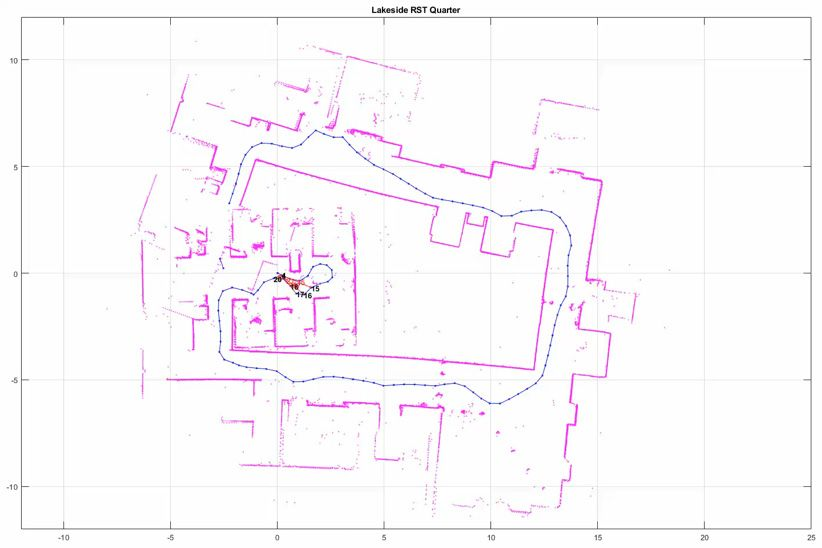
\includegraphics[width=10cm]{pages/algorytm/zdjecia/slam.jpg}
		\caption{Przykład mapowania metodą SLAM\cite{SLAMMat}}
		\label{fig:Rys}
	\end{figure}
	}
\end{itemize}
